% Generated by pysimcount.pffigure -- do not edit; regenerate instead.
% figure: A-measured-by-order -- Suzuki formulas of each order, r from: Measured $r$
% source: results/pf-thesis/results.json
% metric=total gatebase=cz merged
% seed=1 t=n template=simcount synth=pygridsynth
% git_commit=04cd66abb614bdc66fb48e891cef085a299e0ab1 git_dirty=False
% source_sha256=018e0b7603e6fc9f6ee358974f241415a3b93437700847b033937cc1d4250db8
% derived: A-measured-by-order.tex restyled by pysimcount.figuniform: extrapolated points (r from power-law fit) drawn in their series' measured style, style-key legend entries removed; extrapolated n = [13, 20]; source_sha256=b911aa73b857c4d14ab81171d5b6f02f8d101eed9393c95732202d9b4b6551c4
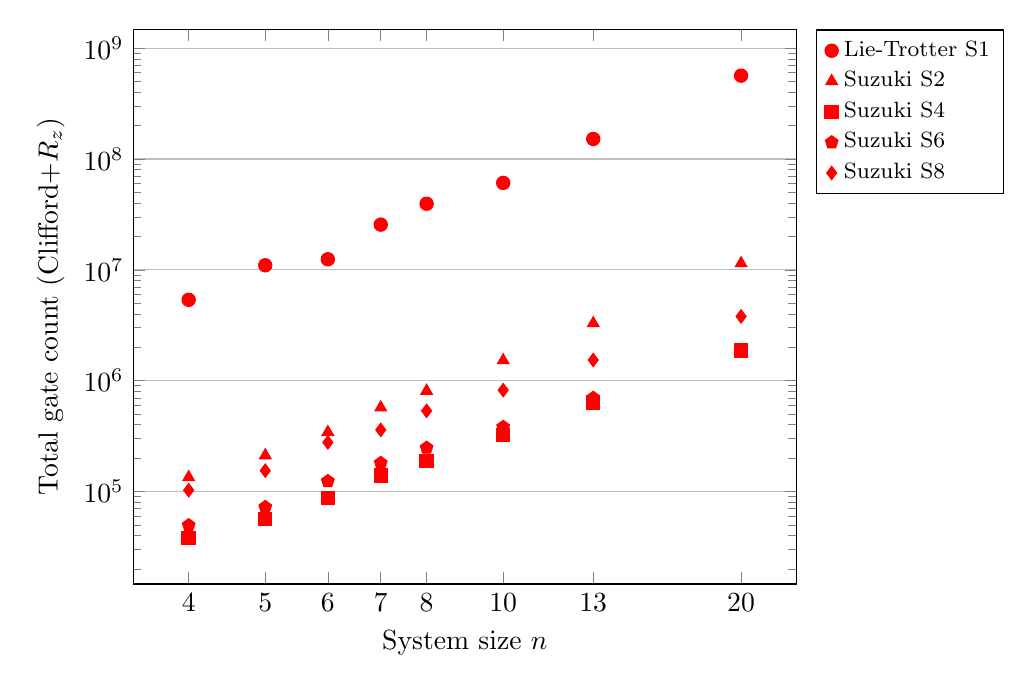
\begin{tikzpicture}
  \begin{loglogaxis}[
    width=10cm,
    xlabel={System size $n$},
    ylabel={Total gate count (Clifford+$R_z$)},
    xtick={4,5,6,7,8,10,13,20},
    xticklabels={4,5,6,7,8,10,13,20},
    ymajorgrids=true,
    legend pos=outer north east,
    legend cell align=left,
    legend style={font=\footnotesize},
  ]
    \addplot[only marks, red, mark=*, mark size=2.4pt, mark options={solid, fill=red}] coordinates {
      (4,5359328)
      (5,10981490)
      (6,12439440)
      (7,25577916)
      (8,39451360)
      (10,60829340)
    };
    \addlegendentry{Lie-Trotter S1}
    % r from power-law fit (extrapolation); one legend entry per series
    \addplot[only marks, red, mark=*, mark size=2.4pt, mark options={solid, fill=red}, forget plot] coordinates {
      (13,151493966)
      (20,564685680)
    };
    \addplot[only marks, red, mark=triangle*, mark size=2.4pt, mark options={solid, fill=red}] coordinates {
      (4,134208)
      (5,211440)
      (6,342432)
      (7,571536)
      (8,807168)
      (10,1523520)
    };
    \addlegendentry{Suzuki S2}
    % r from power-law fit (extrapolation); one legend entry per series
    \addplot[only marks, red, mark=triangle*, mark size=2.4pt, mark options={solid, fill=red}, forget plot] coordinates {
      (13,3289728)
      (20,11429760)
    };
    \addplot[only marks, red, mark=square*, mark size=2.4pt, mark options={solid, fill=red}] coordinates {
      (4,38160)
      (5,56180)
      (6,87768)
      (7,139496)
      (8,188256)
      (10,322240)
    };
    \addlegendentry{Suzuki S4}
    % r from power-law fit (extrapolation); one legend entry per series
    \addplot[only marks, red, mark=square*, mark size=2.4pt, mark options={solid, fill=red}, forget plot] coordinates {
      (13,633880)
      (20,1874080)
    };
    \addplot[only marks, red, mark=pentagon*, mark size=2.4pt, mark options={solid, fill=red}] coordinates {
      (4,49536)
      (5,72240)
      (6,123840)
      (7,180600)
      (8,247680)
      (10,381840)
    };
    \addlegendentry{Suzuki S6}
    % r from power-law fit (extrapolation); one legend entry per series
    \addplot[only marks, red, mark=pentagon*, mark size=2.4pt, mark options={solid, fill=red}, forget plot] coordinates {
      (13,697632)
      (20,1816320)
    };
    \addplot[only marks, red, mark=diamond*, mark size=2.4pt, mark options={solid, fill=red}] coordinates {
      (4,102640)
      (5,153960)
      (6,277128)
      (7,359240)
      (8,533728)
      (10,821120)
    };
    \addlegendentry{Suzuki S8}
    % r from power-law fit (extrapolation); one legend entry per series
    \addplot[only marks, red, mark=diamond*, mark size=2.4pt, mark options={solid, fill=red}, forget plot] coordinates {
      (13,1534468)
      (20,3797680)
    };
  \end{loglogaxis}
\end{tikzpicture}
